\section{Interfaccia utente}

\subsection{Homepage}
La homepage è la prima schermata che l'utente visualizza all'apertura
dell'applicazione. L'elemento principale è un menu a tendina, situato al centro
della pagina: esso contiene una lista di dataset, ognuno dei quali rappresenta
un argomento di studio diverso.
\begin{figure}[ht!]
    \centering
    
\includegraphics[scale=0.6]{template/images/placeholder.png}
    \caption{Menu a tendina}
\end{figure}

Scegliendo un'opzione dal menu, l'utente può visualizzare le informazioni
relative a quel dataset:
\begin{itemize}
    \item Nome del dataset;
    \item Breve descrizione del dataset;
    \item Dimensioni del dataset (numero di righe e colonne);
\end{itemize}
\begin{figure}[ht!]
    \centering
    
\includegraphics[scale=0.6]{template/images/placeholder.png}
    \caption{Informazioni relative a un dataset}
\end{figure}
Inoltre, premendo il pulsante "Avanti", l'utente può avviare il caricamento del
dataset selezionato. Al termine del caricamento, l'utente viene reindirizzato
all'ambiente 3D associato al dataset.
\begin{figure}[ht!]
    \centering
    
\includegraphics[scale=0.6]{template/images/placeholder.png}
    \caption{Pulsante "Avanti"}
    \label{fig:avanti}
\end{figure}

\subsection{Ambiente 3D}
L'ambiente 3D è la schermata principale in cui l'utente può visualizzare i dati
e interagire con essi. La pagina comprende i seguenti elementi:
\begin{itemize}
    \item \textbf{Grafico 3D:} rappresenta il dataset selezionato e consente di
          interagire con esso;
    \item \textbf{Form delle opzioni:} può essere reso visibile premendo
          il pulsante situato in alto a destra. Consente di filtrare i dati in
          base a criteri specifici e modificare le opzioni di visualizzazione;
    \item \textbf{Tabella dei dati:} può essere resa visibile premendo il
          pulsante in basso a sinistra. Mostra il dataset in forma tabellare e
          consente di interagire con esso.
\end{itemize}
\begin{figure}[ht!]
    \centering
    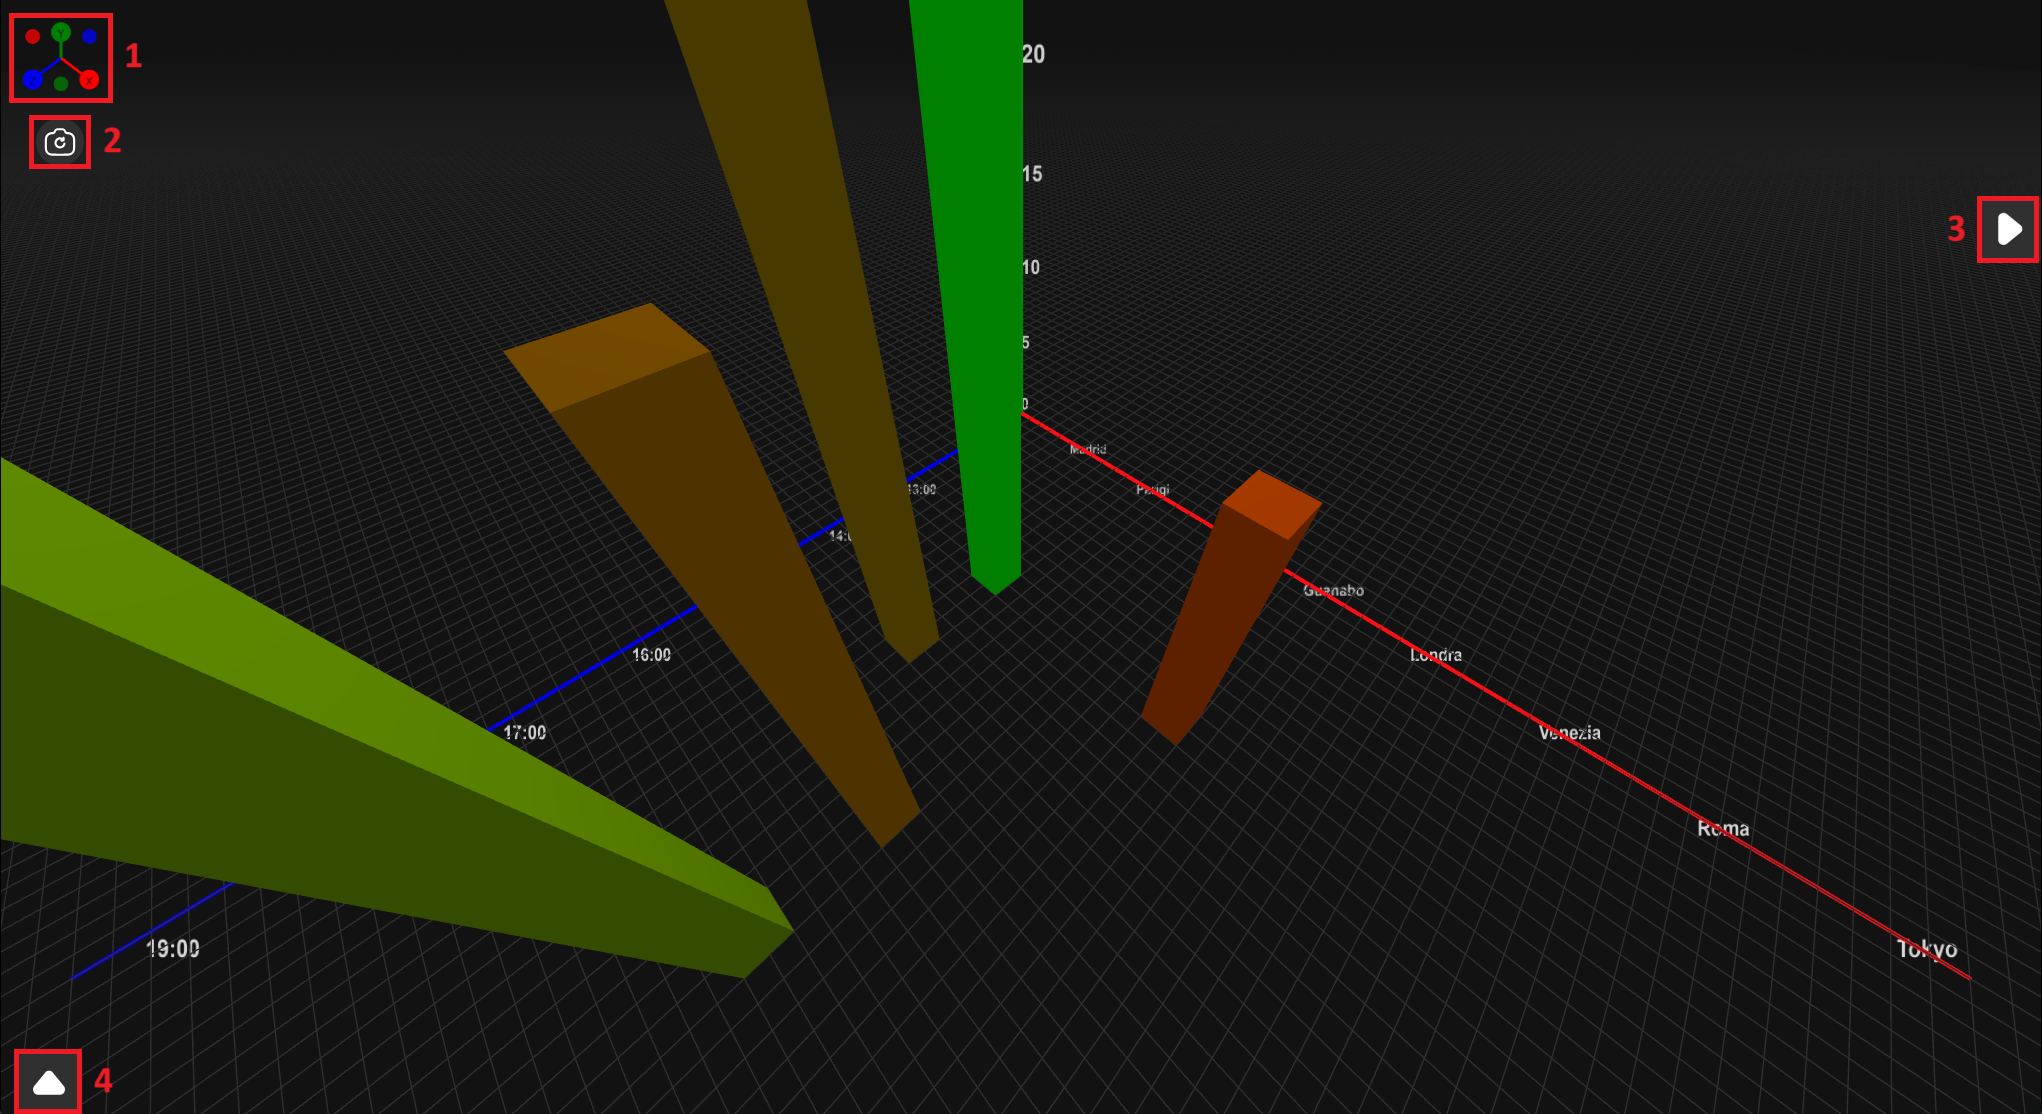
\includegraphics[scale=0.29]{template/images/envpage.png}
    \caption{
        Ambiente 3D con elementi interattivi numerati:\\
        (1) Gizmo;\\
        (2) Pulsante di reset della visualizzazione;\\
        (3) Pulsante per il form delle opzioni;\\
        (4) Pulsante per la tabella.
    }
\end{figure}
\subsubsection{Grafico 3D}
Il grafico 3D è l'elemento centrale dell'ambiente 3D e rappresenta il dataset
selezionato. Ogni barra del grafico rappresenta un valore specifico del
dataset, mentre l'altezza della barra indica il valore stesso. Le barre sono
colorate in base al loro valore, con una scala di colori che va dal rosso
(valori bassi) al verde (valori alti).

\subsubsection{Form delle opzioni}
Il form delle opzioni consente di filtrare i dati in base a criteri specifici e
modificare le opzioni di visualizzazione. Può essere reso visibile oppure
nascosto premendo il pulsante situato in alto a destra nell'ambiente 3D.
Procedendo dall'alto verso il basso, il form è composto da:
\begin{itemize}
    \item Pulsante per filtrare i valori superiori o inferiori (a seconda dell'opzione
          selezionata) al valore medio del dataset;
    \item Campo di input per inserire un numero intero positivo;
    \item Pulsante per filtrare i primi N valori più alti o più bassi (a seconda
          dell'opzione selezionata) del dataset, dove N è il numero inserito nel campo di
          input;
    \item Pulsanti di opzione per scegliere se filtrare i valori più alti o più bassi,
          relativamente a qualunque filtraggio;
    \item Pulsante per rimuovere il filtro applicato;
    \item Pulsanti di opzione per scegliere se visualizzare o meno il piano parallelo al
          piano XZ (base del grafico), che mostra il valore medio del dataset.
\end{itemize}
\begin{figure}[ht!]
    \centering
    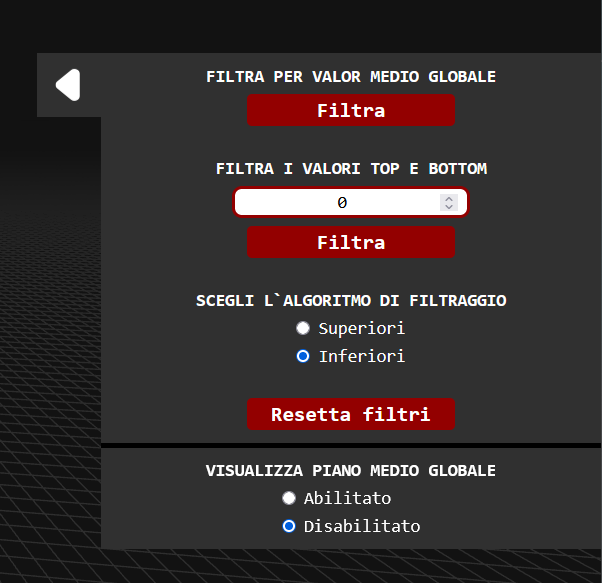
\includegraphics[scale=0.6]{template/images/options.png}
    \caption{Form delle opzioni}
\end{figure}

\subsubsection{Tabella dei dati}
La tabella dei dati mostra il dataset in forma tabellare e consente di
interagire con esso. Può essere resa visibile oppure nascosta premendo il
pulsante situato in basso a sinistra nell'ambiente 3D.\\ La prima colonna
contiene le intestazioni delle righe, che rappresentano le etichette dell'asse
X del grafico. La prima riga contiene le intestazioni delle colonne, che
rappresentano le etichette dell'asse Z del grafico. Le celle della tabella
contengono i valori del dataset e possono assumere colori diversi a seconda che
la corrispondente barra del grafico sia visibile o meno.
\begin{figure}[ht!]
    \centering
    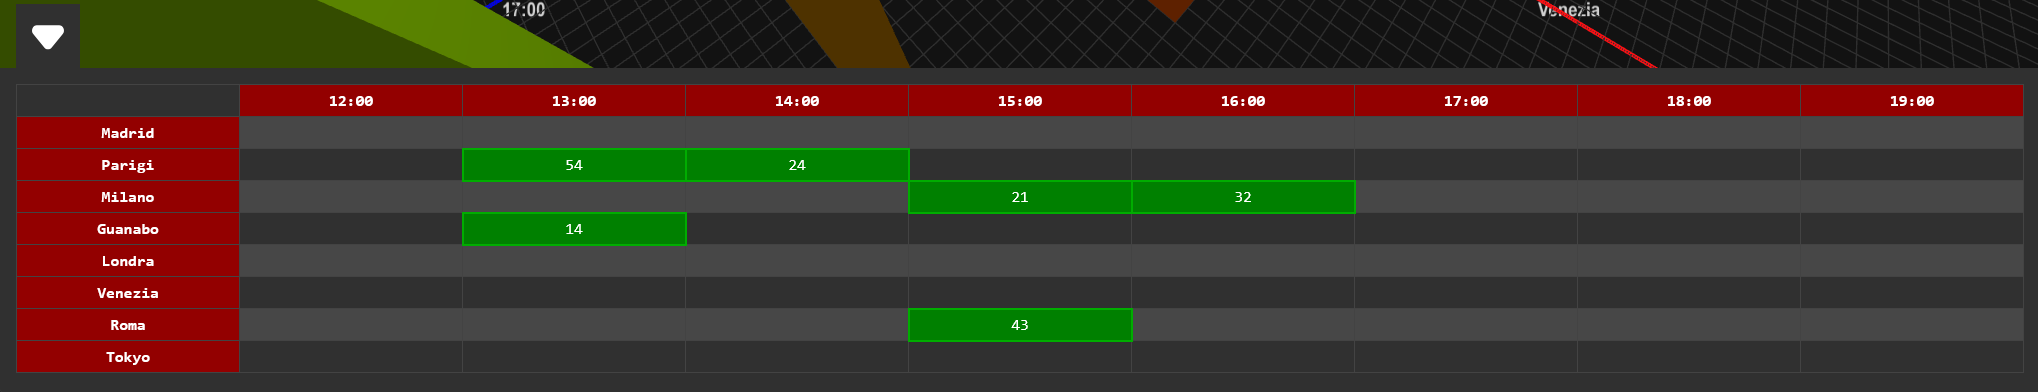
\includegraphics[scale=0.29]{template/images/table.png}
    \caption{Tabella dei dati}
\end{figure}